
\documentclass{beamer}
\usepackage[T1]{fontenc}
\usepackage[polish]{babel}
\usepackage[utf8]{inputenc}
\usepackage{array}
\usepackage{url}
\usetheme{Goettingen}
\setbeamertemplate{frametitle continuation}{}
\titlegraphic{
\includegraphics[width=2cm]{../perebor_5.jpg}}        
\title{Jak komputer uczy się rozwiązywać problemy?}
\author{Robert Trypuz}
\institute{AI po lekcjach}
\date{2024-03-09}

\begin{document}
\frame{\titlepage}
  

\section{INTRO}

\begin{frame}[fragile]
\frametitle{Wprowadzenie}
 \begin{itemize}
\item Wiemy już, że sztuczne inteligencje są programami komputerowymi i że automatyzują procesy myślowe, które zwykle są domeną ludzi.
\item Wspomnieliśmy już, że programowanie sztucznej inteligencji, często określanym jako trenowanie. 
	\begin{itemize}
	\item Proces ten polega na kreowaniu w komputerze specjalnego środowiska, zazwyczaj opartego na sztucznych sieciach neuronowych.
	\item W takim środowisku komputer samodzielnie opracowuje rozwiązania problemów, korzystając z licznych przykładów zawartych w zbiorze treningowym.
	\end{itemize}
\item Ale, jak dokładnie to się odbywa? 
\end{itemize}

\end{frame}

\section{I. Proces uczenia się homo sapiens}

\begin{frame}[fragile]
\frametitle{Jak się uczymy?}
 \begin{itemize}
\item Proces uczenia się komputera, czyli uczenia maszynowego, czerpie inspirację z pewnych aspektów ludzkiego zdobywania wiedzy.
\item Uczymy się poprzez tworzenie wewnętrznych modeli świata. 
\item Termin "model" należy rozumieć, jako pewien uproszczony sposób reprezentacji czegoś innego: 
	\begin{itemize}
	\item na przykład, mapa Lublina jest modelem Lublina.
	\end{itemize}
\item Jest oczywiste, że nie wyczytamy z mapy Lublina wszystkiego o Lublinie; to jedynie uproszczona reprezentacja przestrzennych zależności między budynkami i innymi obiektami. 
\end{itemize}
\end{frame}

\begin{frame}[fragile]
\frametitle{Jak się uczymy?}
\begin{itemize}
\item Nasz mózg przechowuje mnóstwo modeli, czy mentalnych map.
\item Mamy w nim częściowe mapy miast i centrów handlowych, które odwiedziliśmy, mapę naszego mieszkania, i wiele innych. 

                    \begin{figure}[h]
                        \centering
                        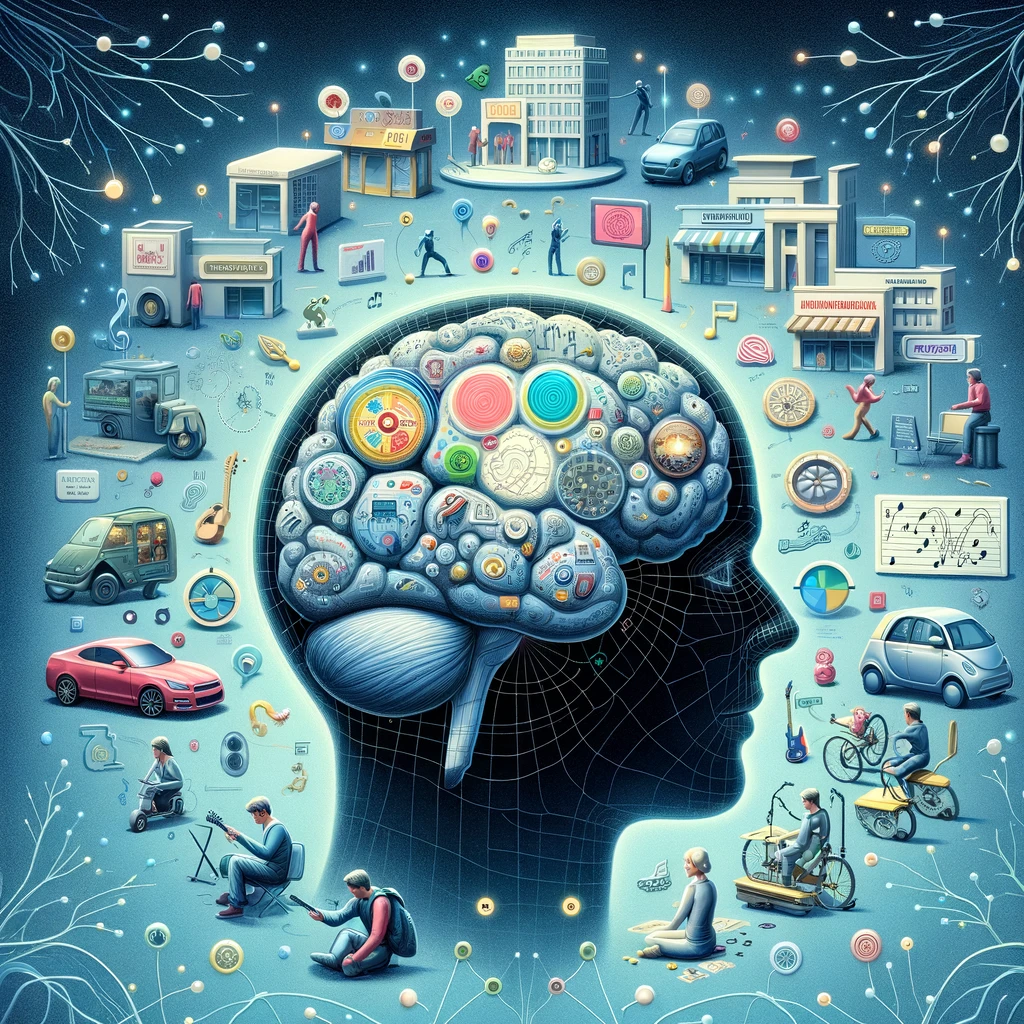
\includegraphics[width=0.5\textwidth]{../../img/mental_maps.png}
                    \end{figure}                    
                    \end{itemize}
\end{frame}

\begin{frame}[fragile]
\frametitle{Jak się uczymy?}
\begin{itemize}
\item Modele jakie posiada mózg mogą być też bardziej dynamiczne; mogą one przypominać “filmy instruktażowe”, np.
	\begin{itemize}
	\item jak używać gorącego kleju
	\item jak prowadzić auto
	\item jak zagrać temat utworu Mr. P.C. Johna Coltrane na gitarze
	\item itd.
	\end{itemize}
\item Uczenie się polega na tworzeniu takich wewnętrznych modeli/mentalnych map. 
\item Nie uświadamiamy sobie istnienia tych modeli. 
	\begin{itemize}
	\item Na przykład każdy z nas, posługujący się językiem polskim, ma model tego języka zapisany w swoim mózgu.
	\item Mamy modele osób, które znamy, ich wyglądu, tonu głosu, ich wrażliwości emocjonalnej - dzięki tym modelom możemy odgrywać w głowie sceny spotkania z nimi, a nawet tworzyć całe dialogi.
	\end{itemize}
\end{itemize}
\end{frame}

\begin{frame}[fragile]
\frametitle{Jak się uczymy?}
\begin{itemize}
\item Uczymy się, czyli tworzymy wewnętrzne modele, od pierwszych miesięcy, obserwując świat wokół siebie, eksperymentując, czyli próbując różnych nowych rzeczy, czy wchodząc w interakcje z innymi.
\item Nasze pierwsze modele nie muszą być od razu poprawne. 
\item Dzięki popełnianym w naszym życiu błędom i \textbf{neuroplastyczności}, czyli zdolności mózgu do zmiany w odpowiedzi na doświadczenia, mamy szansę na ciągłą aktualizację naszych wewnętrznych modeli świata. 
\item To co jest fundamentem procesu uczenia się to: 
	\begin{itemize}
	\item ciągła interakcja z otoczeniem
	\item popełnianie błędów
	\item aktualizacja modeli.
	\end{itemize}
\end{itemize}
\end{frame}

\begin{frame}[fragile]
\frametitle{Jak się uczymy?}
\begin{itemize}
\item Dzięki neuronauce wiemy, że nie rodzimy się jako czysta karta.
	\begin{itemize}
	\item To jaki będzie nasz mózg jest zapisane w naszym genomie jeszcze zanim pojawią się pierwsze jego neurony
	\item A gdy już mózg powstanie, różne jego obszary od samego początku są gotowe do rozpoznawania twarzy ludzi, czy przyswajania języka.
	\end{itemize}
\item Ucząc się sprawiamy, że same neurony jak i połączenia pomiędzy nimi ulegają zmianom (utrwalają się), aby lepiej odzwierciedlać powtarzające się wzorce informacji, które mózg otrzymuje. 
\item Ludzki mózg jest efektywny w rozpoznawaniu wzorców i łączeniu różnorodnych informacji, co umożliwia nam szybkie i efektywne przetwarzanie danych sensorycznych, takich jak obrazy i dźwięki. 
\end{itemize}
\end{frame}

\begin{frame}[fragile]
\frametitle{Uczenie się maszyny, czyli uczenie maszynowe}
\begin{itemize}
\item Uczenie się maszyny, czyli uczenie maszynowe, do pewnego stopnia, naśladuje zdolność ludzkiego mózgu do identyfikacji i nauki wzorców.
\item I tak jak nasze uczenie się opiera się na określonej strukturze naszego mózgu, tak i uczenie maszynowe będzie opierało się na określonej strukturze sztucznych sieci neuronowych. 
\end{itemize}

\end{frame}

\section{II. Jakie inteligentne zadania może wykonać komputer?}

\begin{frame}[fragile]
\frametitle{Co dziś może AI?}
 \begin{itemize}
\item \textbf{Rozpoznawanie obiektów na zdjęciach}
	\begin{itemize}
	\item Komputery są obecnie zdolne do identyfikacji i klasyfikacji obiektów na zdjęciach z dokładnością zbliżoną do zdolności ludzkich. Umożliwia to, między innymi, automatyczne tagowanie fotografii w mediach społecznościowych oraz rozpoznawanie obiektów przez samochody autonomiczne.
	\end{itemize}
\item \textbf{Rozpoznawanie i generowanie mowy} 
	\begin{itemize}
	\item Dzisiejsze technologie umożliwiają komputerom nie tylko rozpoznawanie mowy na poziomie zbliżonym do ludzkiego, ale także generowanie naturalnie brzmiących wypowiedzi. Przykładami tego typu technologii są asystenci głosowi, tacy jak Alexa czy Siri.
	\end{itemize}
\end{itemize}
\end{frame}

\begin{frame}[fragile]
\frametitle{Co dziś może AI?}
\begin{itemize}
\item \textbf{Tłumaczenie tekstów}
	\begin{itemize}
	\item Komputery są w stanie tłumaczyć teksty pomiędzy różnymi językami z imponującą dokładnością i płynnością.
	\end{itemize}
\item \textbf{Tworzenie opowiadań i obrazów} 
	\begin{itemize}
	\item Komputery potrafią również generować kreatywne treści, takie jak opowieści czy obrazy. Dzięki zaawansowanym algorytmom są one w stanie tworzyć realistyczne i spójne narracje, a także generować obrazy na podstawie opisów tekstowych.
	\end{itemize}
\end{itemize}
\end{frame}

\begin{frame}[fragile]
\frametitle{Co dziś może AI?}
\begin{itemize}
\item \textbf{Analiza sentymentu tekstu}
	\begin{itemize}
	\item Komputery mogą analizować tekst pod kątem emocji i tonu wyrażonego przez autora. Przykładowo, mogą określić, czy dana recenzja produktu jest pozytywna czy negatywna.
	\end{itemize}
\item \textbf{Gry i symulacje} 
	\begin{itemize}
	\item Komputery są zdolne do podejmowania strategicznych decyzji w grach i symulacjach, często przewyższając umiejętności ludzkie. Przykładem jest AlphaGo, program komputerowy, który pokonał mistrza gry w Go.
	\end{itemize}
\end{itemize}
\end{frame}

\begin{frame}[fragile]
\frametitle{Co dziś może AI?}
\begin{itemize}
\item \textbf{Diagnostyka medyczna}
	\begin{itemize}
	\item Dzięki uczeniu maszynowemu, komputery mogą wspierać diagnozowanie chorób, analizując wyniki badań obrazowych i laboratoryjnych z precyzją porównywalną lub nawet przewyższającą umiejętności lekarzy.
	\end{itemize}
\item \textbf{Automatyzacja procesów biznesowych} 
	\begin{itemize}
	\item Komputery potrafią automatyzować wiele rutynowych zadań, takich jak obsługa klienta (chatboty) czy podejmowanie decyzji o przyznaniu kredytu.
	\end{itemize}
\end{itemize}

\end{frame}

\section{III. Czego potrzebujemy, aby komputer mógł się uczyć?}

\begin{frame}[fragile]
\frametitle{Czego potrzebuje AI, aby się uczyć?}
 \begin{itemize}
\item Aby umożliwić komputerowi naukę wykonania konkretnego zadania konieczne jest spełnienie trzech warunków.
\item Dla łatwiejszego zrozumienie, wyjaśnijmy rzecz na przykładzie znanego problemu/zadania rozpoznawania ręcznie pisanych cyfr od 0 do 9. 
\end{itemize}
\end{frame}

\begin{frame}[fragile]
\frametitle{Czego potrzebuje AI, aby się uczyć?}
\begin{itemize}
\item \textbf{1) Dane treningowe}
\item W przypadku rozpoznawania ręcznie pisanych cyfr, dane treningowe stanowią zbiór obrazów przedstawiających cyfry od 0 do 9. Zazwyczaj potrzebujemy setek obrazków każdej cyfry, aby komputer mógł nauczyć się różnorodności form i stylów pisania. Każdy obrazek powinien być opisany, co w tym kontekście oznacza przypisanie mu odpowiedniej cyfry, której dotyczy. Te opisy, zwane etykietami (ang. label), umożliwiają komputerowi zrozumienie, co jest przedstawione na każdym obrazku. 
\end{itemize}
\end{frame}

\begin{frame}[fragile]
\frametitle{Czego potrzebuje AI, aby się uczyć?}
\begin{itemize}
\item \textbf{2) Sztuczna sieć neuronowa}
\item Aby komputer mógł przetwarzać i uczyć się z danych treningowych, potrzebujemy środowiska, w którym będzie się to odbywać, czyli sztucznej sieci neuronowej. Sztuczne sieci neuronowe są zdolne do nauki i rozpoznawania wzorców w danych, co jest kluczowe w procesie uczenia maszynowego. 
\end{itemize}
\end{frame}

\begin{frame}[fragile]
\frametitle{Czego potrzebuje AI, aby się uczyć?}
\begin{itemize}
\item \textbf{3) Metoda oceny}
\item Konieczne jest posiadanie metody, która pozwala ocenić, czy sztuczna sieć neuronowa uczy się poprawnie i czy osiągnęła pożądany poziom dokładności.
 Metoda zmiany. Konieczne jest posiadanie metody zmiany ustawień/parametrów sieci w przypadku błędnego jej działania. 
\end{itemize}
\end{frame}

\begin{frame}[fragile]
\frametitle{Przykład}
\begin{itemize}
\item Załóżmy więc, że pierwszy punkt jest spełniony i posiadamy odpowiednie dane treningowe. Na przykład możemy skorzystać z dostępnej publicznie bazy danych obrazków MNIST zawierającej ręcznie pisane cyfry, składającej się z 70 000 przykładów!

                    \begin{figure}[h]
                        \centering
                        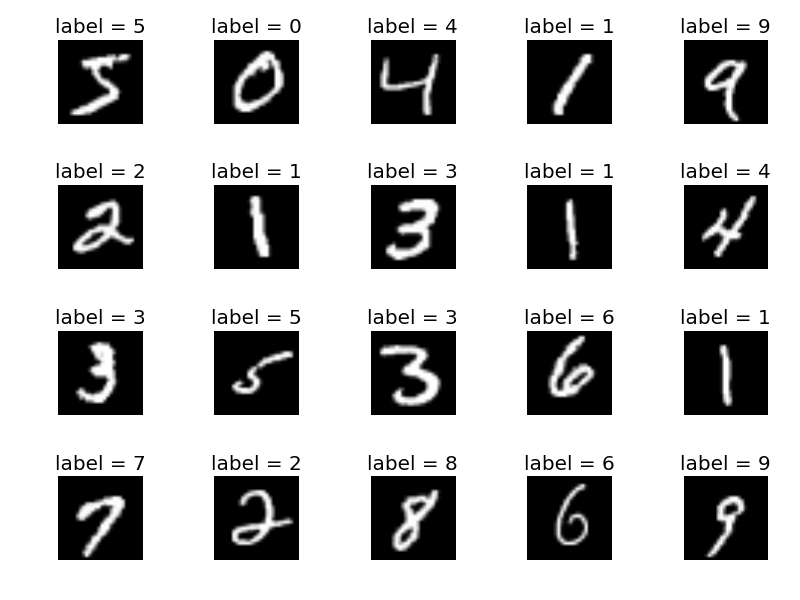
\includegraphics[width=0.5\textwidth]{../../img/mnist_plot.png}
                    \end{figure}                    
                    \item Jak jednak zbudować sztuczną sieć neuronową i co to w ogóle jest? 
\end{itemize}

\end{frame}

\section{IV. Od neuronu biologicznego do sztucznej sieci neuronowej}

\begin{frame}[fragile]
\frametitle{Neuron biologiczny}
 \begin{itemize}
\item Sposób działania sztucznego neuronu czerpie swoją inspirację z neuronu biologicznego.
\item Biologiczny neuron to komórka, która odbiera, generuje i przekazuje impulsy. 

                    \begin{figure}[h]
                        \centering
                        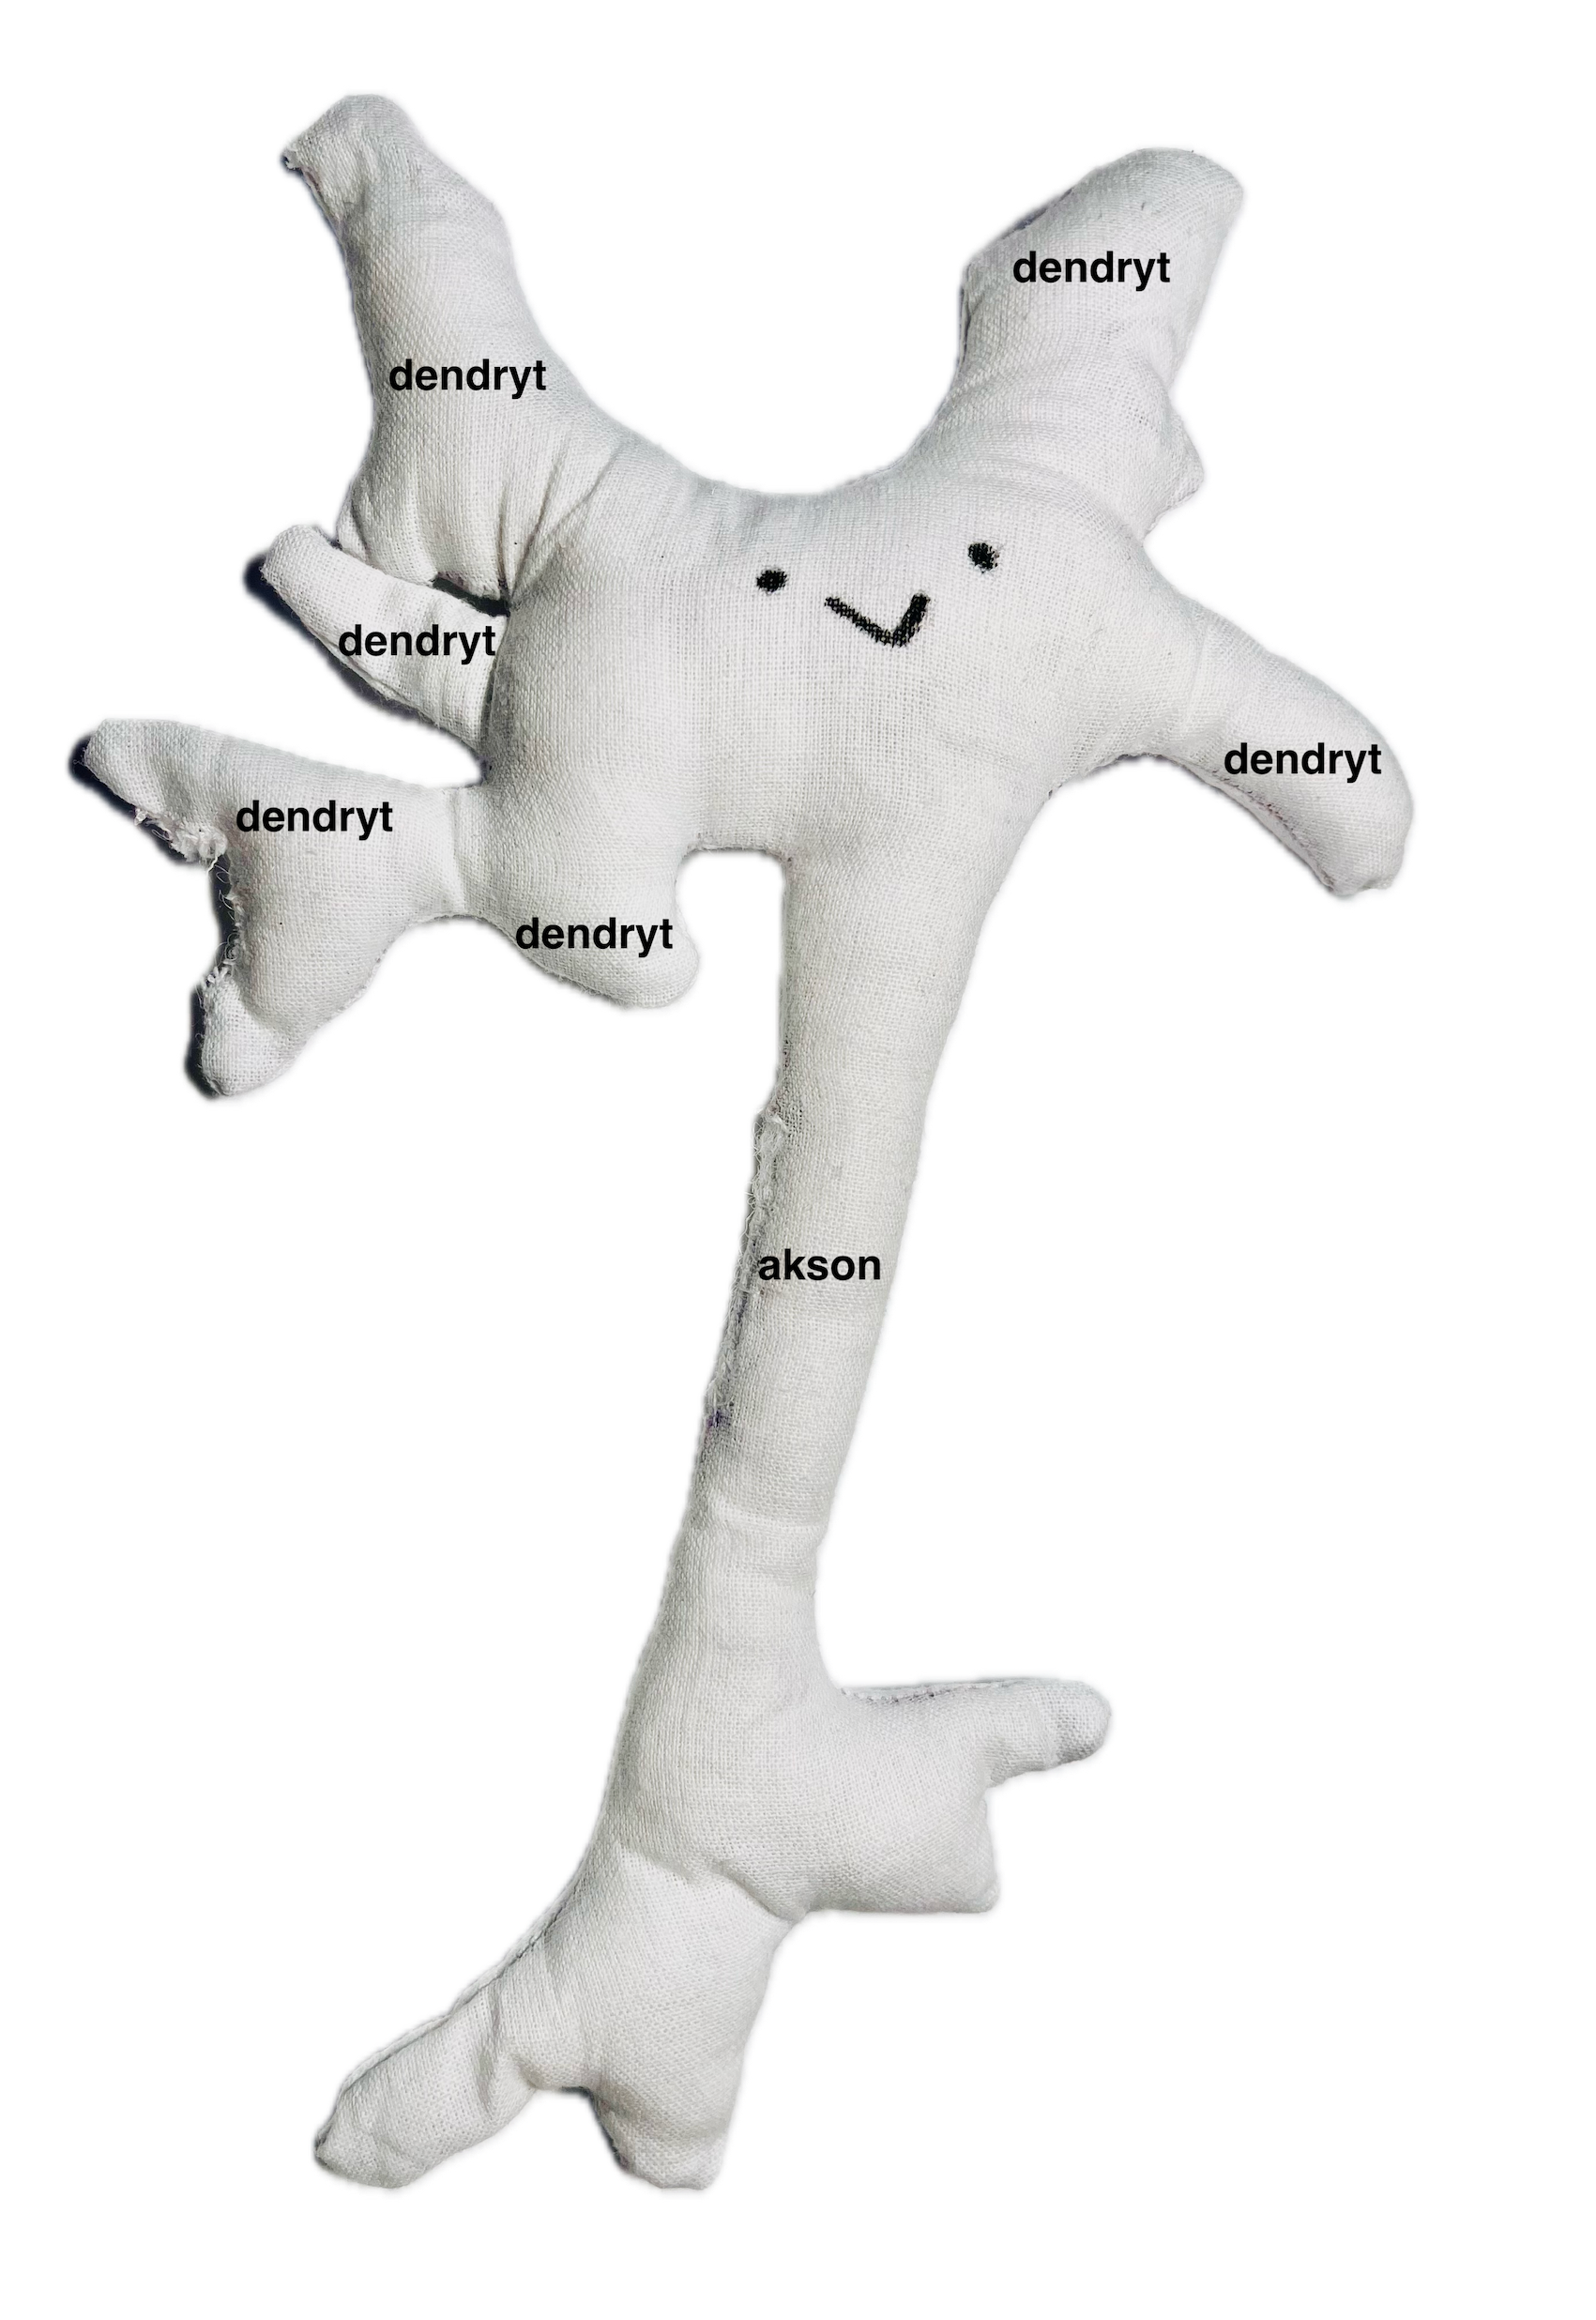
\includegraphics[width=0.5\textwidth]{../../img/neuron_mt2.png}
                    \end{figure}                    
                    \end{itemize}
\end{frame}

\begin{frame}[fragile]
\frametitle{Neuron biologiczny}
\begin{itemize}
\item Dendryty, czyli wypustki neuronu, odbierają impulsy od innych neuronów lub od receptorów zmysłów.
\item Gdy suma impulsów osiągnie pewien próg, neuron generuje impuls elektryczny, który przemieszcza się aksonem do innych komórek przez synapsy 
	\begin{itemize}
	\item gdy impuls elektryczny dociera do końca neuronu na granicę synapsy i "chce" przejść do innego neuronu napotyka wyzwanie: przerwa między neuronami, zwana szczeliną synaptyczną, nie przewodzi impulsu elektrycznego
	\item w tym momencie w grę wchodzą substancje chemiczne zwane neurotransmiterami, które neuron wysyła do tej szczeliny; przemieszczają się one przez szczelinę synaptyczną i łączą się z receptorami na neuronie odbierającym i wówczas generowany jest nowy impuls elektryczny
	\end{itemize}
\end{itemize}
\end{frame}

\begin{frame}[fragile]
\frametitle{Sztuczny neuron}
\begin{itemize}
\item Sztuczny neuron: ma coś na kształt dendrytów - są to liczby wejściowe.  Są one następnie, podobnie jak impulsy neuronu biologicznego, sumowane i przekazywane do specjalnej funkcji aktywacji, która decyduje jak silna będzie reakcja neuronu.

                    \begin{figure}[h]
                        \centering
                        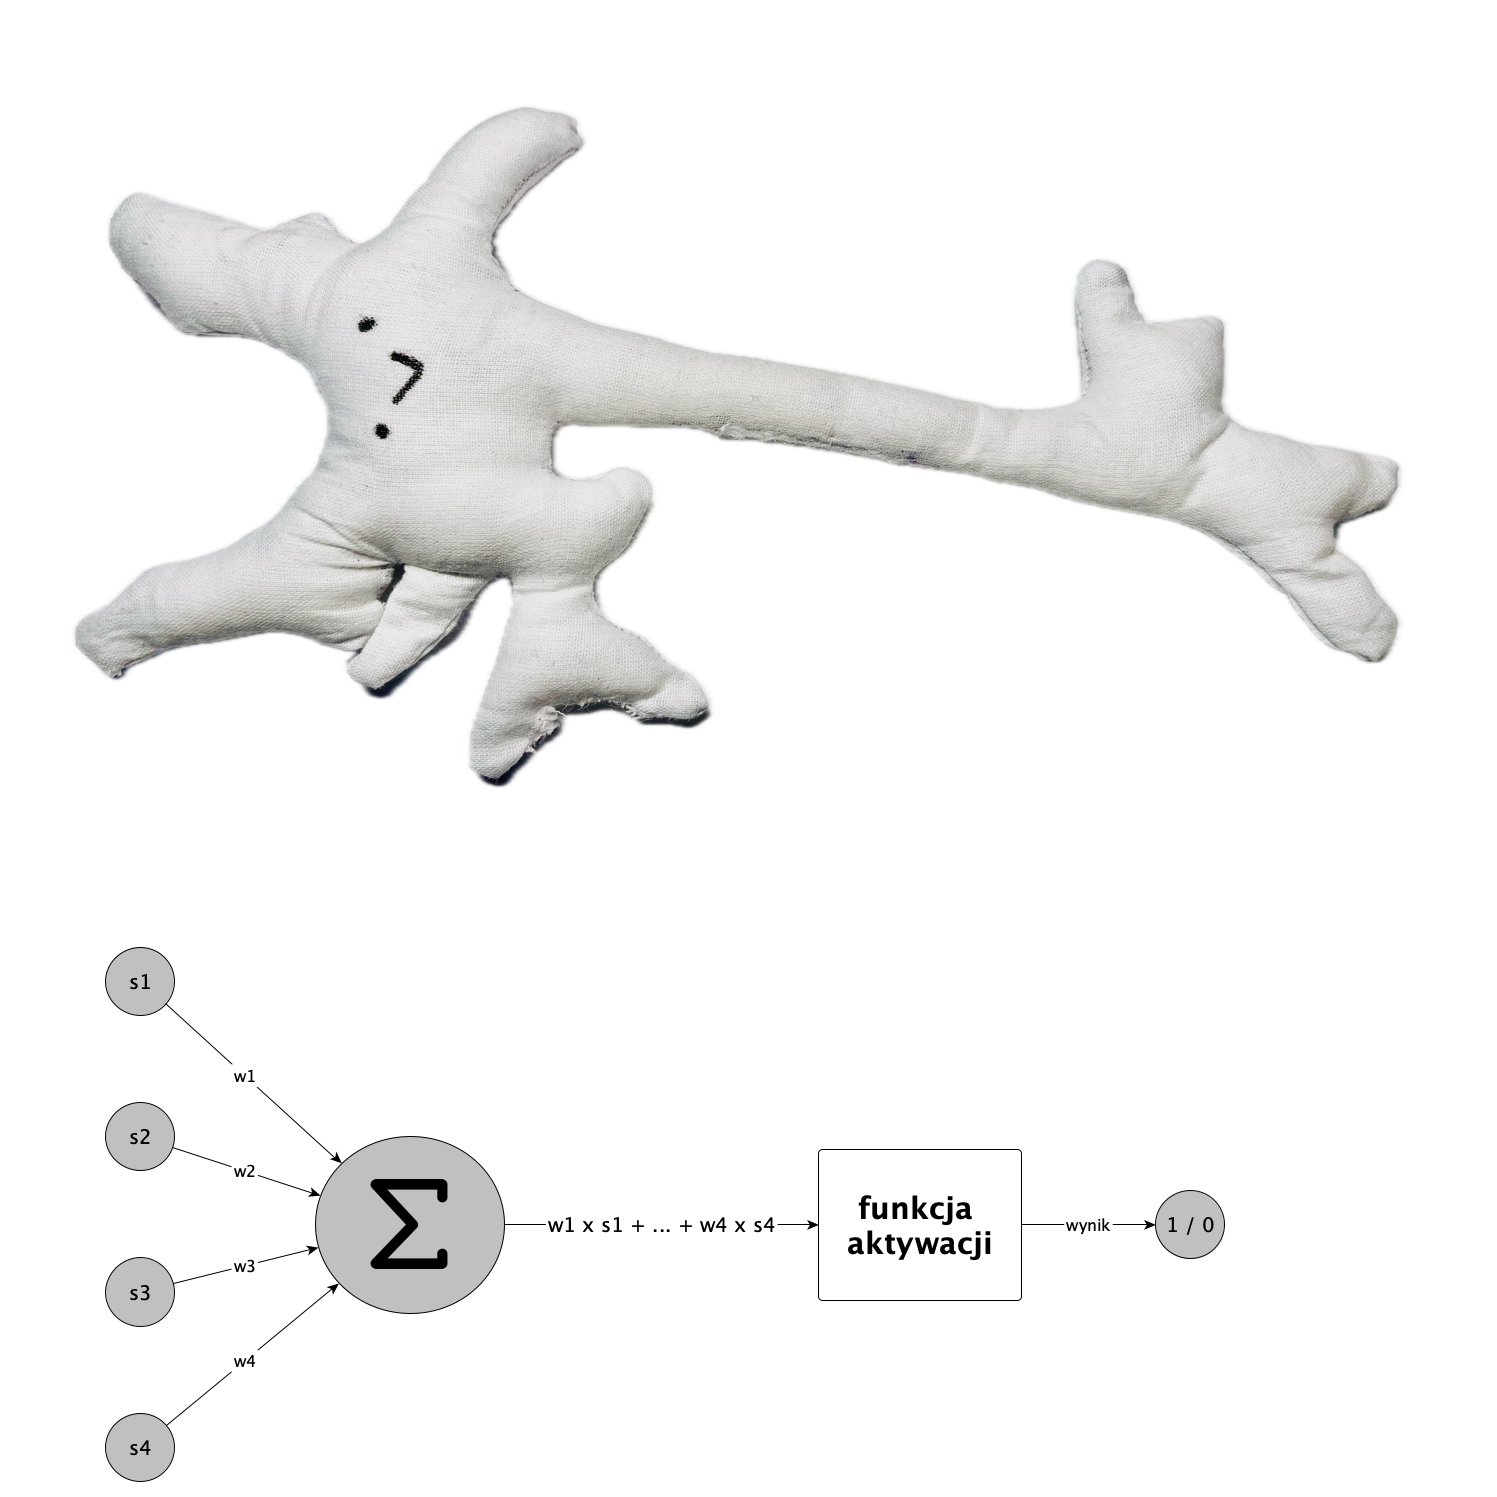
\includegraphics[width=0.5\textwidth]{../../img/neuron.png}
                    \end{figure}                    
                    \end{itemize}
\end{frame}

\begin{frame}[fragile]
\frametitle{Sztuczny neuron}
\begin{itemize}
\item Sztuczny neuron przyjmuje impulsy `s1, ..., s4`, waży je, czyli przemnaża je przez wartości wag: `w1, ..., w4`, a następnie sumuje ważone impulsy: `w1 x s1 + w2 x s2 + w3 x s3 + w4 x s4` i przekazuje je do funkcji aktywacji wyliczającej wynik `1` lub `0`.
\item Na przykład, taka funkcja aktywacji może określić próg, wartości `0.5`, i jeśli suma impulsów przekroczy go, to zwracana jest wartość `1`, co odpowiada powstaniu impulsu elektrycznego w neuronie biologicznym, albo `0`, co oznaczałoby brak impulsu. 
\item Aktywacja sztucznego neuronu nie musi być binarna `0` albo `1`. Może być też zdefiniowana np. jako wartość z przedziału `[0,1]` - czym mocniejszy sygnał wejściowy, tym większa wartość aktywacji. 
\end{itemize}
\end{frame}

\begin{frame}[fragile]
\frametitle{Sztuczny neuron}
\begin{itemize}
\item Podobnie jak neuron biologiczny nie traktuje wszystkich dendrytów tak samo "poważnie", tzn. impulsy od jednych dendrytów traktuje jako ważniejsze niż od innych, sztuczny neuron również waży swoje dane wejściowe.
\item To ważenie w praktyce polega na przemnożeniu impulsu przez ułamek, co skutkuje zmniejszeniem wartości takiego sygnału. Na przykład przemnażając sygnał o wartości `1` przez `0.5` otrzymamy `0.5`, czyli wartość sygnału zmniejszyła się o połowę. 
\end{itemize}
\end{frame}

\begin{frame}[fragile]
\frametitle{Sieć neuronowa}
\begin{itemize}
\item Oczywiście jeden neuron nie jest w stanie wiele zdziałać. Aby rozwiązywać inteligentne zadania, neurony muszą być połączone w sieć.
\item Sztuczna sieć neuronowa złożona z 15 neuronów: 

                    \begin{figure}[h]
                        \centering
                        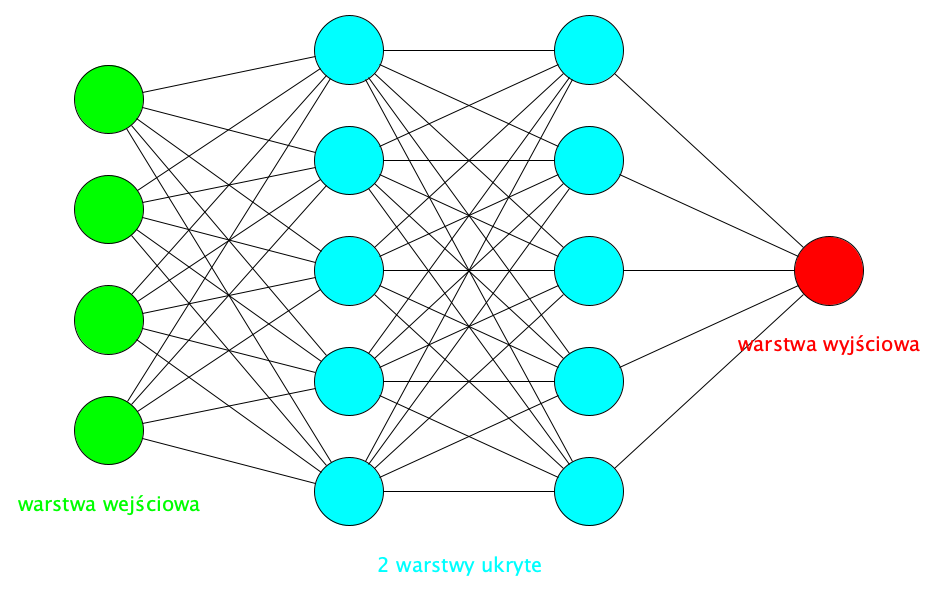
\includegraphics[width=0.5\textwidth]{../../img/nn.png}
                    \end{figure}                    
                    \item Gdy opisujemy sztuczne sieci neuronowe zwykle wyróżniamy warstwy neuronów. Mamy więc warstwę wejściową, która przyjmuje wartości liczbowe wyrażające impulsy, mamy warstwę wyjściową oraz dowolnie wiele warstw pomiędzy warstwą wejściową i wyjściową, które nazywamy warstwami ukrytymi. 
\end{itemize}
\end{frame}

\begin{frame}[fragile]
\frametitle{Sieć jest modelem matematycznym}
\begin{itemize}
\item Ważne jest, aby zrozumieć, że neurony w sztucznych sieciach neuronowych, które się dziś używa, nie są niczym fizycznym; są to po prostu jednostki obliczeniowe, a sama sieć jest modelem matematycznym.
\end{itemize}
\end{frame}

\begin{frame}[fragile]
\frametitle{Neuron jako ekspert}
\begin{itemize}
\item Możemy metaforycznie myśleć o każdym neuronie w sieci jako o ekspercie.

                    \begin{figure}[h]
                        \centering
                        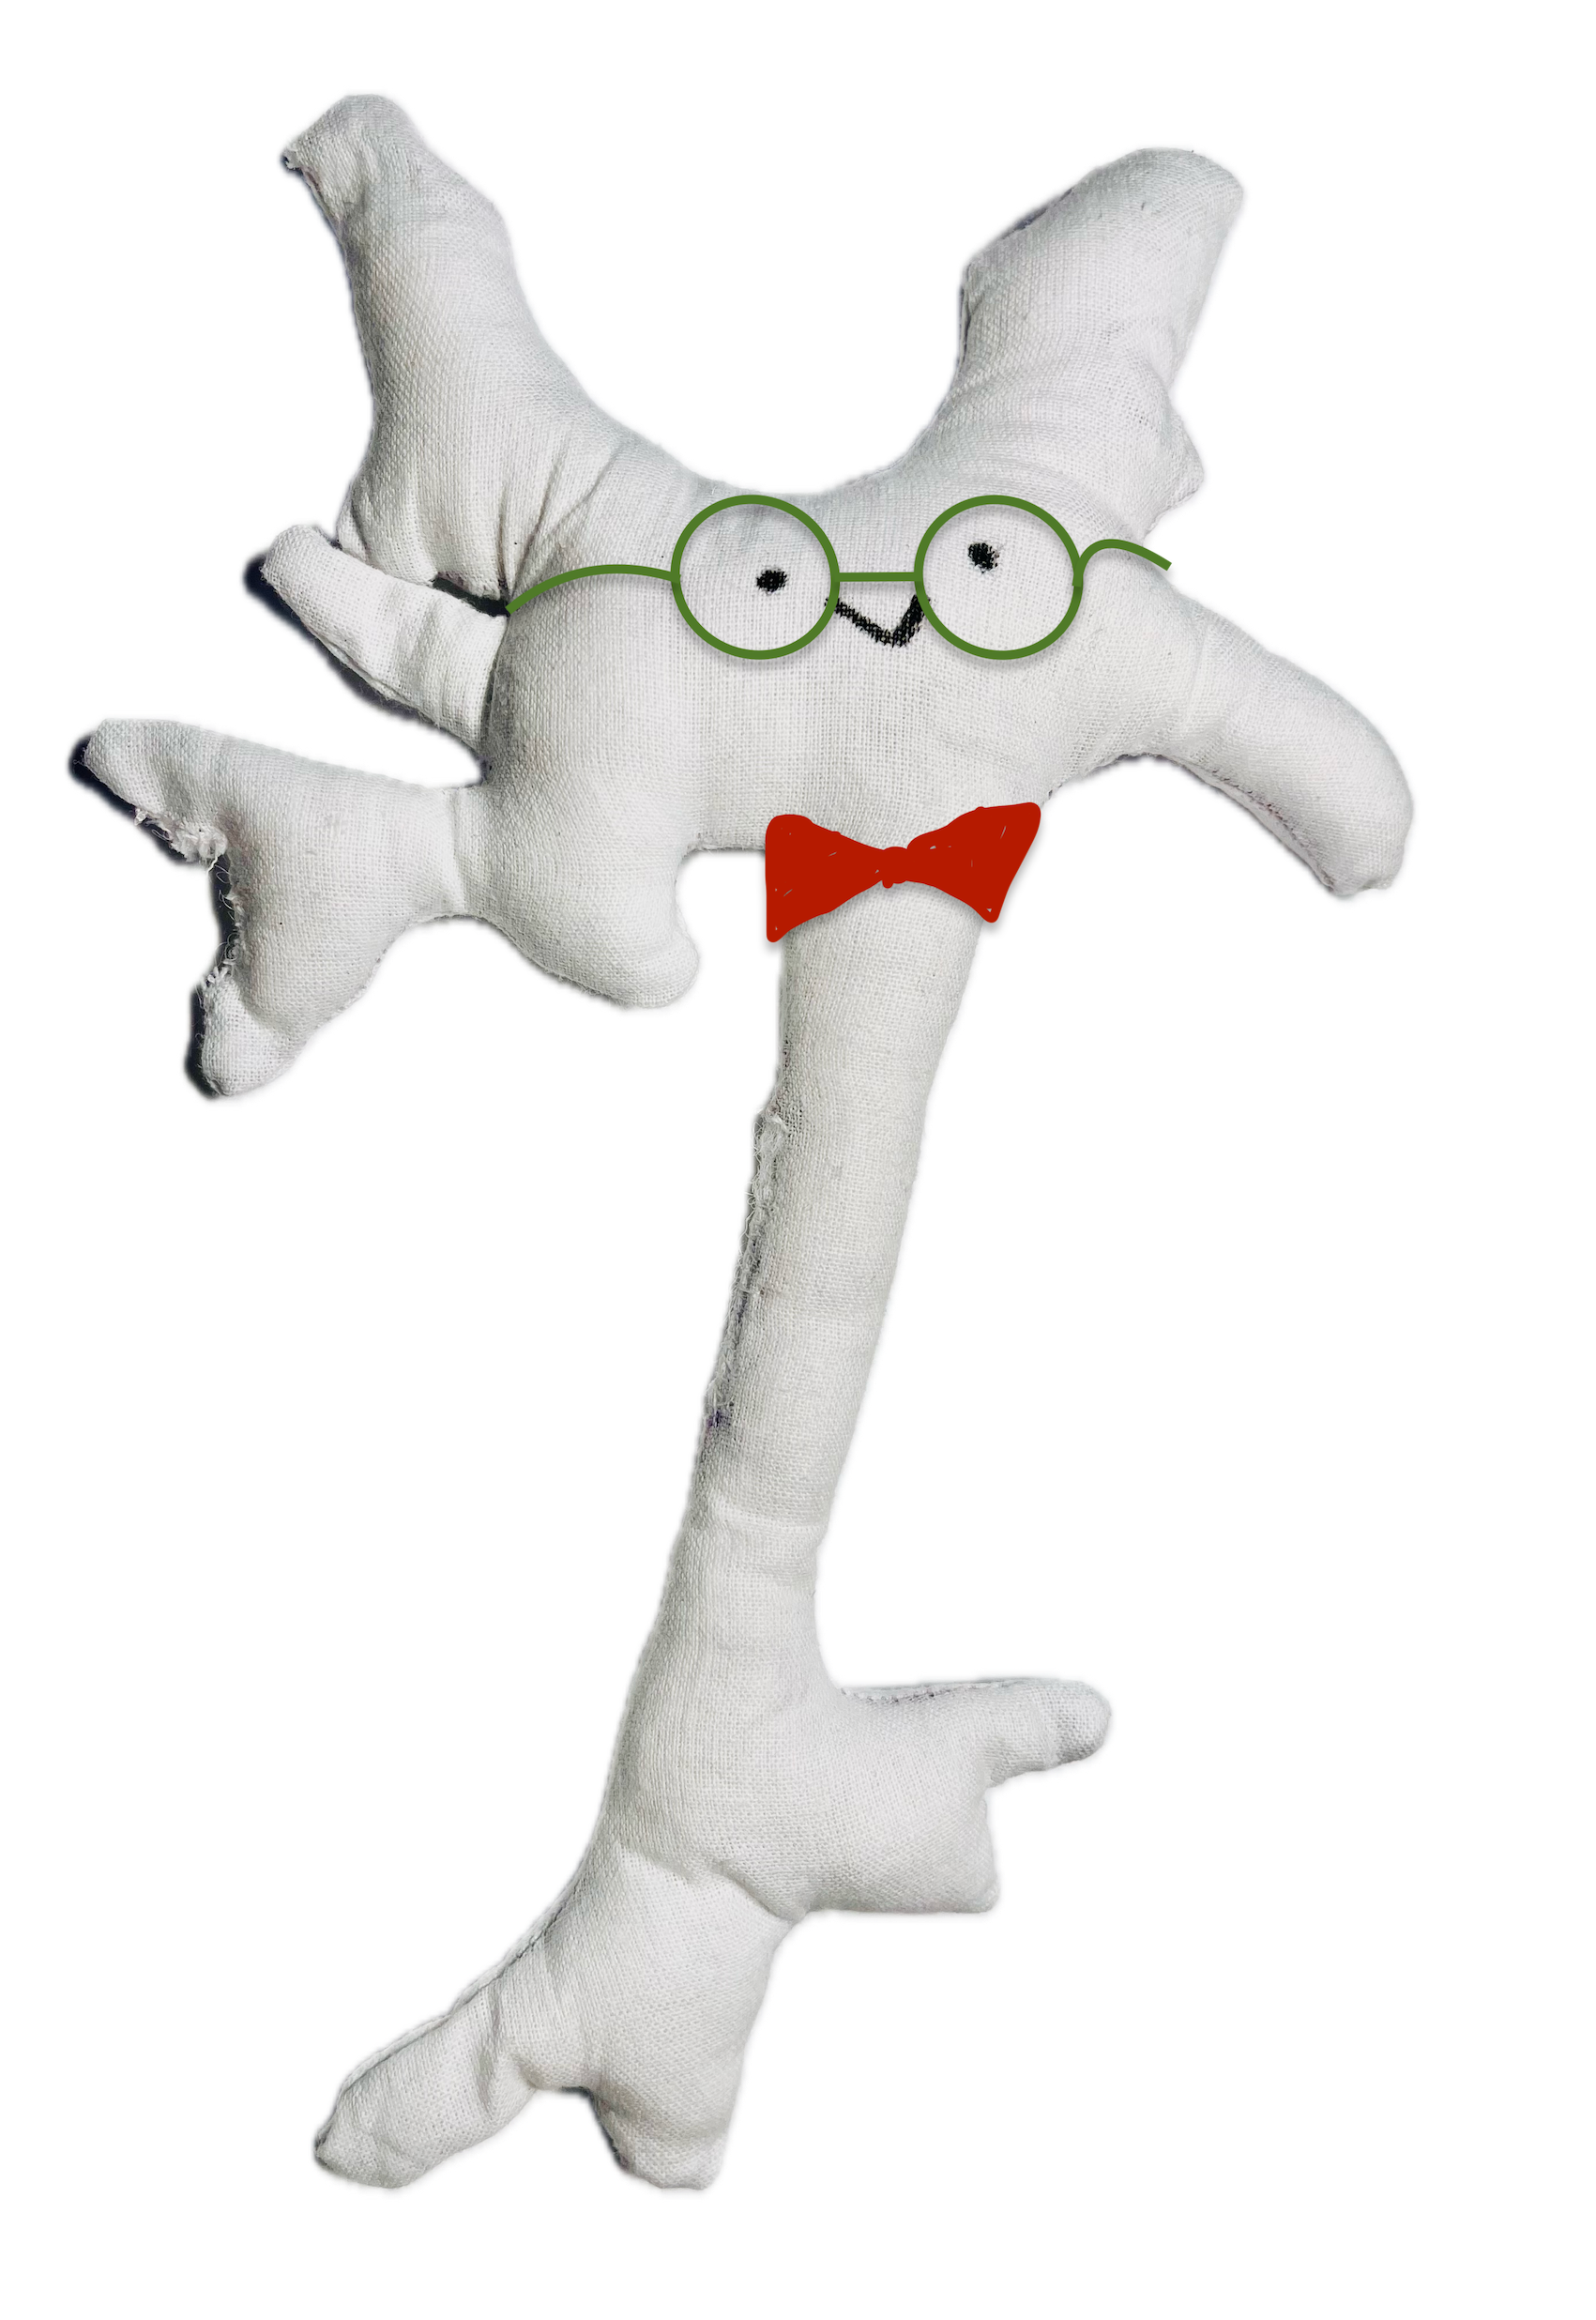
\includegraphics[width=0.5\textwidth]{../../img/neuron_ekspert.png}
                    \end{figure}                    
                    \end{itemize}
\end{frame}

\begin{frame}[fragile]
\frametitle{Neuron jako ekspert}
\begin{itemize}
\item I tak...
	\begin{itemize}
	\item W warstwie wejściowej będą neurony/eksperci, które przyjmują bezpośrednio dane wejściowe.
	\item Następnie przekazują je do neuronów/ekspertów w pierwszej warstwie ukrytej.
	\item Ci analizują te dane i w pewnej przetworzonej formie przekazują je dalej do ekspertów w drugiej warstwie ukrytej.
	\item Ci czynią podobnie: analizują i przetwarzają.
	\item Rezultat swoich “przemyśleń” ostatnia warstwa ukryta przekazuje do ekspertów z warstwy wyjściowej, którzy muszą podjąć decyzję, która zależy od typu problemu.
	\end{itemize}
\end{itemize}

\end{frame}

\section{V. Przykład sieci}

\begin{frame}[fragile]
\frametitle{Przykład}
 \begin{itemize}
\item Wróćmy do problemu rozpoznawania ręcznie pisanych cyfr od 0 do 9.

                    \begin{figure}[h]
                        \centering
                        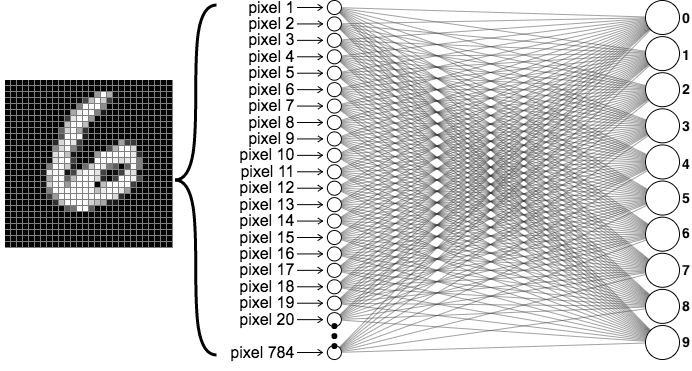
\includegraphics[width=0.5\textwidth]{../../img/mnist_1layer.png}
                    \end{figure}                    
                    \item W takim przypadku, działanie (wcześniej nauczonej) sztucznej sieci neuronowej będzie wyglądało następująco. 
\end{itemize}
\end{frame}

\begin{frame}[fragile]
\frametitle{Przykład}
\begin{itemize}
\item Warstwa wejściowa neuronów/ekspertów przyjmie dane wejściowe w postaci obrazka (na którym jest cyfra "6" - jak na obrazku powyżej).
\item Ponieważ obrazki składają się z pikseli, czyli pojedynczych kwadracików, to nasza sieć musi mieć w warstwie wejściowej tyle neuronów ile jest pikseli. Jeśli mamy obrazki o wielkości 28 na 28 pikseli (czyli mamy szachownicę 28x28), to wszystkich pikseli jest 28 razy 28, czyli 784. Jeśli mamy obrazki czarno-białe, to każdy piksel może być reprezentowany za pomocą liczby od 0 - 255, gdzie 0 oznacza czarny, a 255 biały, a wszystko pomiędzy będzie skalą szarości. 
\end{itemize}
\end{frame}

\begin{frame}[fragile]
\frametitle{Przykład}
\begin{itemize}
\item Czyli w warstwie wejściowej mamy 784 neuronów/ekspertów i każdy przyjmuje "impuls" w postaci wartość koloru (0-255) od dokładnie jednego piksela. Następnie każdy neuron/ekspert z warstwy wejściowej przekazuje te dane do każdego neuronu/eksperta z pierwszej warstwy ukrytej. Każdy ekspert z pierwszej warstwy ukrytej waży po swojemu informacje, które do niego dochodzą, przetwarza je i przekazuje do każdego eksperta w kolejnej warstwie ukrytej. Proces ten kontynuowany jest aż do momentu, gdy neurony/eksperci z ostatniej warstwy ukrytej przekażą swoje przetworzone wartości do warstwy wyjściowej.
\item W warstwie wyjściowej dla tego problemu mamy 10 neuronów/ekspertów, każdy jest ekspertem od jednej z cyfr 0-9. Pierwszy od “0”, drugi od “1”, i ostatni od “9”. Każdy z nich wyrazi swoją opinię, która przez sieć zostanie przedstawiona ostatecznie w postaci prawdopodobieństwa, czyli stopnia pewności. Można więc powiedzieć, że pierwszy ekspert oceni prawdopodobieństwo, że na obrazku jest cyfra "0", drugi oceni prawdopodobieństwo obecności cyfry "1", a ostatni - cyfry "9". Jeśli sieć jest dobrze wytrenowana, to neuron - ekspert odpowiedzialny za cyfrę "6" - powinien wyrazić się z najwyższą pewnością. 
\end{itemize}

\end{frame}

\section{VI. Jak uczy się sztuczna sieć neuronowa?}

\begin{frame}[fragile]
\frametitle{Procesu uczenia sztucznej sieci neuronowej}
 \begin{itemize}
\item Celem procesu uczenia sztucznej sieci neuronowej jest nauczenie jej prawidłowego odwzorowywania danych na ich etykiety, na przykład, odwzorowania obrazków na odpowiadające im cyfry od 0 do 9.
\item Aby to osiągnąć, każdy neuron/ekspert, zostaje wyposażony w zestaw wag, przy czym każda waga odpowiada jednemu sygnałowi wejściowemu, w naszym przykładzie, jednemu pikselowi obrazka. 
\item Na początku procesu uczenia każdy neuron inicjuje wartości wag losowo. Zazwyczaj są to bardzo małe wartości, co można interpretować jako początkowy sceptycyzm neuronu co do jakości sygnałów wejściowych. 
\end{itemize}
\end{frame}

\begin{frame}[fragile]
\frametitle{Procesu uczenia sztucznej sieci neuronowej}
\begin{itemize}
\item Uczenie ma dwa kierunki, nazwijmy je: czerwony i zielony.

                    \begin{figure}[h]
                        \centering
                        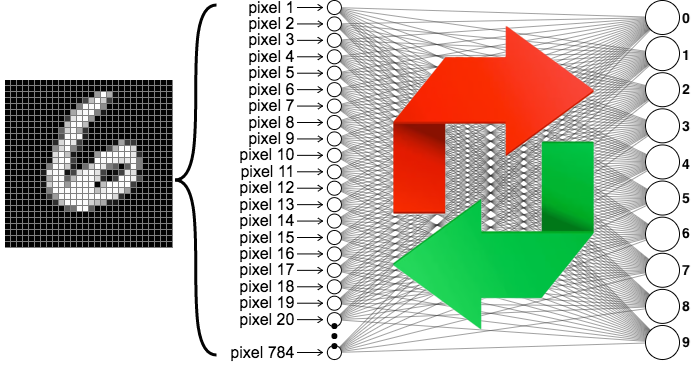
\includegraphics[width=0.5\textwidth]{../../img/mnist_1layer with arrows.png}
                    \end{figure}                    
                    \item Kierunki uczenia: 
	\begin{itemize}
	\item strzałka czerwona to propagacja "do przodu"
	\item strzałka zielona to propagacja wsteczna.
	\end{itemize}
\end{itemize}
\end{frame}

\begin{frame}[fragile]
\frametitle{Propagacja "do przodu"}
\begin{itemize}
\item Kierunek czerwony (propagacja "do przodu") to prosty proces przyjmowania przez neurony kolejnych warstw wartości od wszystkich neuronów z warstwy poprzedniej, ważenie tych sygnałów (czyli przemnożenie tych sygnałów przez wagi), określenie poziomu aktywacji w oparciu o tę ważoną sumę sygnałów i przekazanie impulsu dalej.
	\begin{itemize}
	\item W tym konkretnym przykładzie, warstwa wyjściowa, składa się z 10 neuronów/ekspertów i ma ciekawą funkcję aktywacji, która nazywa się softmax.
	\item Każdy neuron/ekspert warstwy wyjściowej przyjmie impuls od każdego neuronu ostatniej warstwy wyjściowej, wygeneruje ważoną sumę i przekaże tę sumę do funkcji sofmax.
	\item Softmax na tej podstawie, przypisze każdemu neuronowi prawdopodobieństwo/stopień pewności.
	\item Największa suma będzie miała najwyższe prawdopodobieństwo.
	\end{itemize}
\end{itemize}
\end{frame}

\begin{frame}[fragile]
\frametitle{Propagacja "do przodu"}
\begin{itemize}
\item Na przykład, wartości sumy dla kolejnych neuronów, odpowiadających za rozpoznawanie cyfr 0, 1, ...9, mogą być następujące:
	\begin{itemize}
	\item 2, 1, 0, 5, 1, 0, 0, 2, 1, 4
	\end{itemize}
\item a softmax przekształci je na prawdopodobieństwa (sposób wyliczenia pomijam): 
	\begin{itemize}
	\item 3.2\%, 1.1\%, 0.4\%, 64.8\%, 1.1\%, 0.4\%, 0.4\%, 3.2\%, 1.1\%, 23.8\%.
	\end{itemize}
\item Oznacza to, że sieć jest prawie w 65\% pewna, że na obrazku jest cyfra 3, w około 24\% że to 9, itd. 
\end{itemize}
\end{frame}

\begin{frame}[fragile]
\frametitle{Funkcja straty}
\begin{itemize}
\item Jeśli założymy, że obrazek na wejściu przedstawia "6" (jak to jest w przykładzie powyżej), to sieć dokonała błędnej predykcji: "3".
\item Kiedy sieć dokona predykcji, od razu dowiaduje się, czy była ona poprawna czy nie, dzięki specjalnej funkcji straty, która porównuje prognozę sieci (3) z oczekiwaną odpowiedzią (6). 
\item Funkcję straty można wyobrazić sobie jako miernik rozbieżności między prognozami modelu a rzeczywistymi etykietami. 
\item Jeśli prognozy modelu są bliskie prawdziwym etykietom, strata jest niska. Jeśli są one bardzo rozbieżne, strata jest wysoka. Funkcja straty jest metodą oceny jak sieć radzi sobie podczas uczenia. 
\end{itemize}
\end{frame}

\begin{frame}[fragile]
\frametitle{Propagacja wsteczna}
\begin{itemize}
\item Tutaj wartość błędu odbiera tzw. optymalizator, którego zadaniem jest wprowadzenie zmian w wartości wag, które posiadają neurony/eksperci.
\item Innymi słowy, optymalizator znajduje neurony odpowiedzialne za powstanie błędu i odpowiednio zmienia wartości wag, którymi posługiwały się te neurony podczas błędnej predykcji. 
\item Optymalizator dzięki specjalnemu \textbf{algorytmowi “propagacji wstecznej”} dokładnie wie, które neurony są odpowiedzialne za błędną predykcję i w jaki sposób zmienić ich wagi. 
\item Algorytm “propagacji wstecznej” to jedno z największych osiągnięć w rozwoju AI. Dzięki niemu proces uczenia się sztucznych sieci neuronowych może być w pełni zautomatyzowany. 
\end{itemize}
\end{frame}

\begin{frame}[fragile]
\frametitle{Iteracyjny process uczenia się sieci neuronowej}
\begin{itemize}
\item Proces uczenia się sztucznych sieci neuronowych jest iteracyjny: sieć przyjmuje kolejny obrazek, dokonuje predykcji (kierunek czerwony), następnie koryguje wagi (kierunek zielony) i tak dalej. Dzięki temu procesowi iteracyjnemu, sieć poprawia swoje predykcje w każdej iteracji, zbliżając się do celu prawidłowego rozpoznawania cyfr na obrazkach.
\item Dodajmy, że wagi, którymi dysponują neurony, nazywa się również parametrami sieci. Suma wszystkich wag/parametrów wszystkich neuronów sieci jest często miarą jej złożoności. 
\end{itemize}
\end{frame}

\begin{frame}[fragile]
\frametitle{SNARC - pierwsza samoucząca się sztuczna sieć neuronowa}
\begin{itemize}
\item Pierwsza samoucząca się sztuczna sieć neuronowa, SNARC (ang. \textit{Stochastic Neural Analog Reinforcement Calculator}), była złożona z 40 fizycznych neuronów takiej oto postaci:

                    \begin{figure}[h]
                        \centering
                        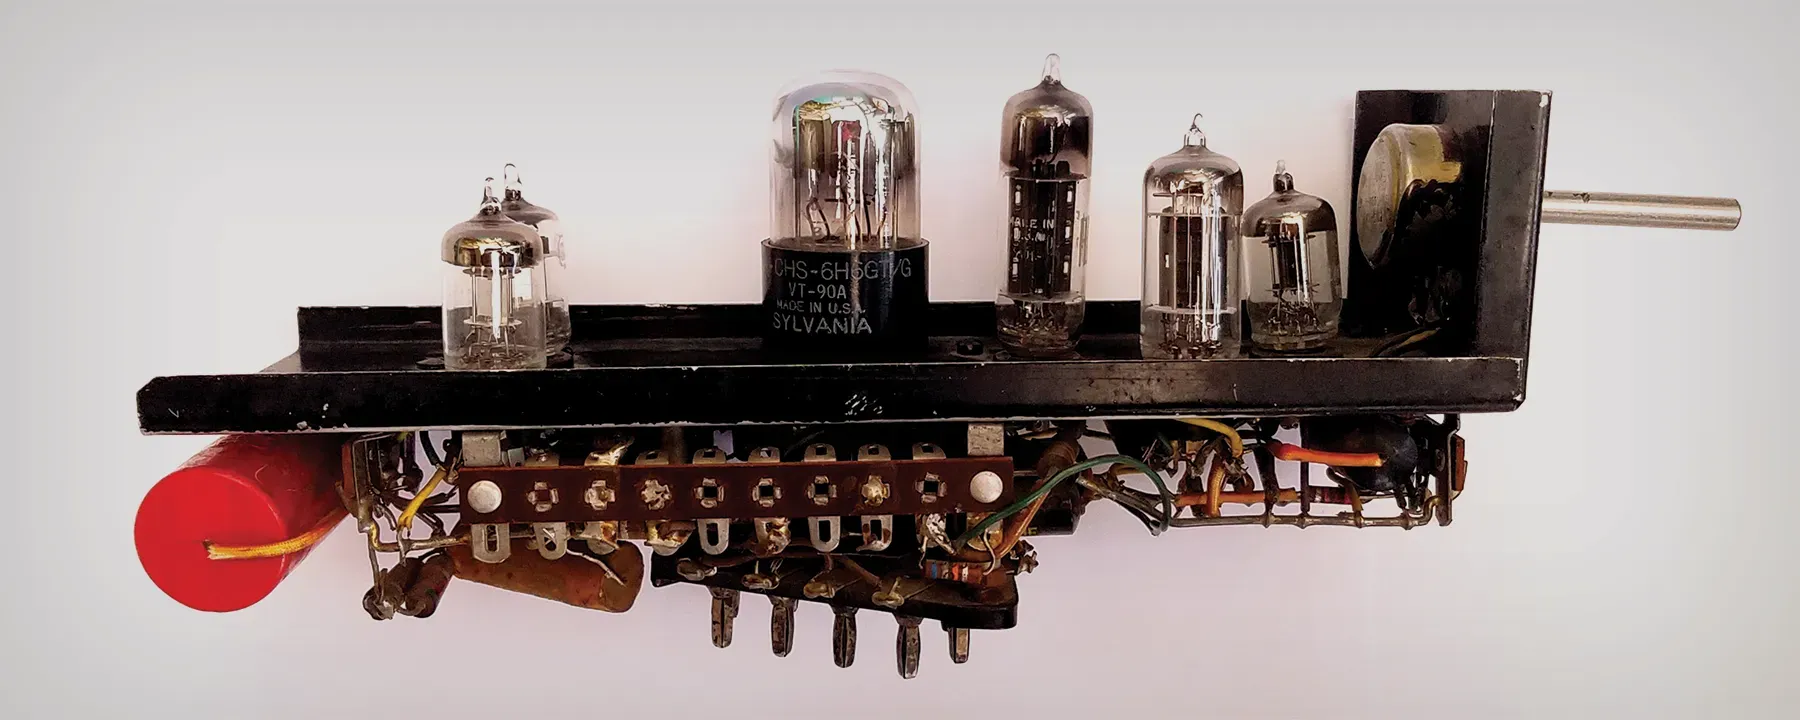
\includegraphics[width=0.5\textwidth]{../../img/the-scientist-foundations-original-the-first-artifical-intelligence-x.png}
                    \end{figure}                    
                    \item Ten wystający po prawej stronie bolec, to potencjometr pokręcając którym zmniejszało się, albo zwiększało wagę neuronu. 
\end{itemize}

\end{frame}

\section{OUTRO}

\begin{frame}[fragile]
\frametitle{Powiedzieliśmy, że...}
 \begin{itemize}
\item Proces uczenia maszynowego, do pewnego stopnia, naśladuje zdolność ludzkiego mózgu do identyfikacji i nauki wzorców. I tak jak nasze uczenie się opiera się na określonej strukturze naszego mózgu, tak i uczenie maszynowe będzie opierało się na określonej strukturze sztucznych sieci neuronowych.
\item Komputery obecnie potrafią wykonywać wiele inteligentnych zadań, takich jak: rozpoznawanie obiektów na zdjęciach, generowanie mowy, tłumaczenie tekstów, tworzenie kreatywnych treści, analiza sentymentu, podejmowanie decyzji w grach, diagnostyka medyczna oraz automatyzacja procesów biznesowych. 
\end{itemize}
\end{frame}

\begin{frame}[fragile]
\frametitle{Powiedzieliśmy, że...}
\begin{itemize}
\item Aby nauczyć komputer wykonywania zadania, potrzebne są odpowiednie dane treningowe, sztuczna sieć neuronowa oraz metody oceny skuteczności uczenia oraz korekty parametrów sieci.
\item Sztuczne sieci neuronowe, inspirowane działaniem neuronów biologicznych, składają się z warstw neuronów, które przetwarzają i ważą dane wejściowe, a następnie przekazują je przez funkcje aktywacji do kolejnych warstw, aby finalnie podjąć decyzję w warstwie wyjściowej. 
\item Uczenie sztucznej sieci neuronowej polega na iteracyjnym procesie, w którym sieć dokonuje predykcji poprzez ważenie sygnałów wejściowych przy użyciu wstępnie losowo inicjowanych wag, a następnie koryguje te wagi za pomocą optymalizatora i algorytmu propagacji wstecznej, aby zminimalizować błąd pomiędzy prognozami a rzeczywistymi etykietami. 
\end{itemize}
\end{frame}


\end{document}
    